\documentclass[11pt]{article} % use larger type; default would be 10pt


%%% PAGE DIMENSIONS
\usepackage[top=1in, bottom=1in, left=1in, right=1in]{geometry} % to change the page dimensions
 
%%% PACKAGES
\usepackage{graphicx} % support the \includegraphics command and options
\usepackage{amsfonts}
\usepackage{amsmath}
\usepackage{tikz}
\usepackage{graphicx}
\usepackage{color}
 
%%% The "real" document content comes below...

\title{CS 134 \\ \emph{Problem Set 3}}
\author{Xiner Zhou}
\date{\today} % Activate to display a given date or no date (if empty),
        

\begin{document}
 
\maketitle

 \paragraph{1. Centrality (Jackson 2.2.4).}
 
 \begin{itemize}
\item[\textbf{a.}] Compute the degree centrality of each of the nodes in network $B$. 
 \end{itemize}

\textcolor{red}{Solution:} 

%%%%%%%%% Network B
 
\begin{center}
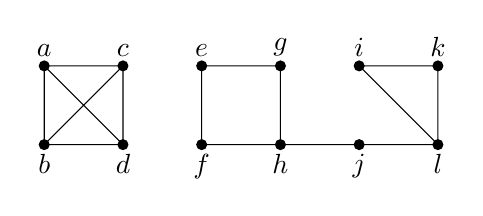
\begin{tikzpicture} [scale=1]
 
\coordinate [label=above:{$a$}] (a) at (0,1);
\coordinate [label=below:{$b$}] (b) at (0,0);
\coordinate [label=above:{$c$}] (c) at (1,1);
\coordinate [label=below:{$d$}] (d) at (1,0);
\coordinate [label=above:{$e$}] (e) at (2,1);
\coordinate [label=below:{$f$}] (f) at (2,0);
\coordinate [label=above:{$g$}] (g) at (3,1);
\coordinate [label=below:{$h$}] (h) at (3,0);
\coordinate [label=above:{$i$}] (i) at (4,1);
\coordinate [label=below:{$j$}] (j) at (4,0);
\coordinate [label=above:{$k$}] (k) at (5,1);
\coordinate [label=below:{$l$}] (l) at (5,0);

\fill (a) circle (2pt);
\fill (b) circle (2pt);
\fill (c) circle (2pt);
\fill (d) circle (2pt);
\fill (e) circle (2pt);
\fill (f) circle (2pt);
\fill (g) circle (2pt);
\fill (h) circle (2pt);
\fill (i) circle (2pt);
\fill (j) circle (2pt);
\fill (k) circle (2pt);
\fill (l) circle (2pt);

\draw (a)--(d)--(c)--(b)--(a)--(c)--(d)--(b);
\draw (h)--(f)--(e)--(g)--(h)-- (j)--(l)--(k)--(i)--(l);

\end{tikzpicture}
\end{center}



The nodes $a,b,c,d,h,l$ all have degree 3, and the nodes $e,f,g,i,j,k$ all have degree 2. Therefore,
$$degree \  centrality(a)=degree \  centrality(b)$$
$$=degree \  centrality(c)=degree  \   centrality(d)$$
$$=degree \  centrality(h)=degree \   centrality(l) $$
$$=\frac{3}{12-1}=\frac{3}{11}$$

$$degree \   centrality(e)=degree \   centrality(f)=degree \   centrality(g) $$
$$=degree  \  centrality(i)=degree  \  centrality(j)=degree \   centrality(k) $$
$$=\frac{2}{12-1}=\frac{2}{11}$$


\begin{enumerate} 
\item[\textbf{b.}]Compute the closeness centrality of node $d$ in network  $$(\{a,b,c,d\},\{ab,ac,ad,bc,cd\}).$$
 \end{enumerate}
 

\textcolor{red}{Solution:} 

%%%%%%%%% Network B
 
\begin{center}
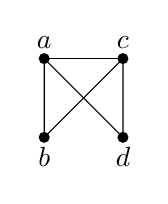
\begin{tikzpicture} [scale=1]
 
\coordinate [label=above:{$a$}] (a) at (0,1);
\coordinate [label=below:{$b$}] (b) at (0,0);
\coordinate [label=above:{$c$}] (c) at (1,1);
\coordinate [label=below:{$d$}] (d) at (1,0);
 

\fill (a) circle (2pt);
\fill (b) circle (2pt);
\fill (c) circle (2pt);
\fill (d) circle (2pt);
 

\draw (a)--(b)--(c)--(d) ;
\draw (a)--(c) ;
\draw (a)--(d) ;

\end{tikzpicture}
\end{center}
 

$$closeness \   centrality(d)=\displaystyle \frac{1}{\frac{dist(d,a)+dist(d,b)+dist(d,c)}{3}}$$
$$=\frac{1}{\frac{1+2+1}{3}}$$
$$=\frac{3}{4}$$








































\paragraph{2. Betweenness Centrality.} Compute the betweenness centrality of each of the nodes in the network $(\{a,b,c,d,e,f\}, \{ab,bc,cd,ce,df,ef\})$. 

%%%%%%%%% Network  
 
\begin{center}
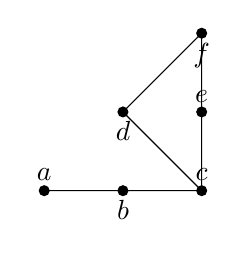
\begin{tikzpicture} [scale=1]

\coordinate [label=above:{$a$}] (a) at (0,0);
\coordinate [label=below:{$b$}] (b) at (1,0);
\coordinate [label=above:{$c$}] (c) at (2,0);
\coordinate [label=below:{$d$}] (d) at (1,1);
\coordinate [label=above:{$e$}] (e) at (2,1);
\coordinate [label=below:{$f$}] (f) at (2,2);

\fill (a) circle (2pt);
\fill (b) circle (2pt);
\fill (c) circle (2pt);
\fill (d) circle (2pt);
\fill (e) circle (2pt);
\fill (f) circle (2pt);
 
\draw (a)--(b)--(c)--(e)--(f)--(d)--(c) ;
\end{tikzpicture}
\end{center}


\textcolor{red}{Solution:} 

\begin{itemize}
	\item 
$betweenness \  centrality(a)=\frac{1}{10} \times $ 
$$ (\frac{P_a(b,c)}{P(b,c)}+\frac{P_a(b,d)}{P(b,d)}+\frac{P_a(b,e)}{P(b,e)}+\frac{P_a(b,f)}{P(b,f)}+\frac{P_a(c,d)}{P(c,d)}+\frac{P_a(c,e)}{P(c,e)}+\frac{P_a(c,f)}{P(c,f)}\frac{P_a(d,e)}{P(d,e)}+\frac{P_a(d,f)}{P(d,f)}+\frac{P_a(e,f)}{P(e,f)})$$
$$=\frac{1}{10} \times (0+0+0+0+0+0+0+0+0+0) = 0$$
	\item 
$betweenness \  centrality(b)=\frac{1}{10} \times $ 
$$ (\frac{P_b(a,c)}{P(a,c)}+\frac{P_b(a,d)}{P(a,d)}+\frac{P_b(a,e)}{P(a,e)}+\frac{P_b(a,f)}{P(a,f)}+\frac{P_b(c,d)}{P(c,d)}+\frac{P_b(c,e)}{P(c,e)}+\frac{P_b(c,f)}{P(c,f)}\frac{P_b(d,e)}{P(d,e)}+\frac{P_b(d,f)}{P(d,f)}+\frac{P_b(e,f)}{P(e,f)})$$
$$=\frac{1}{10} \times (1+1+1+\frac{1}{2}+0+0+0+0+0+0) = \frac{7}{20}$$
	\item 
$betweenness \  centrality(c)=\frac{1}{10} \times $ 
$$ (\frac{P_c(a,b)}{P(a,b)}+\frac{P_c(a,d)}{P(a,d)}+\frac{P_c(a,e)}{P(a,e)}+\frac{P_c(a,f)}{P(a,f)}+\frac{P_c(b,d)}{P(b,d)}+\frac{P_c(b,e)}{P(b,e)}+\frac{P_c(b,f)}{P(b,f)}\frac{P_c(d,e)}{P(d,e)}+\frac{P_c(d,f)}{P(d,f)}+\frac{P_c(e,f)}{P(e,f)})$$
$$=\frac{1}{10} \times (0+1+1+1+1+1+1+\frac{1}{2}+0+0) = \frac{13}{20}$$
 
	\item 
$betweenness \  centrality(d)=\frac{1}{10} \times $ 
$$ (\frac{P_d(a,b)}{P(a,b)}+\frac{P_d(a,c)}{P(a,c)}+\frac{P_d(a,e)}{P(a,e)}+\frac{P_d(a,f)}{P(a,f)}+\frac{P_d(b,c)}{P(b,c)}+\frac{P_d(b,e)}{P(b,e)}+\frac{P_d(b,f)}{P(b,f)}\frac{P_d(c,e)}{P(c,e)}+\frac{P_d(c,f)}{P(c,f)}+\frac{P_d(e,f)}{P(e,f)})$$
$$=\frac{1}{10} \times (0+0+0+\frac{1}{2}+0+0+\frac{1}{2}+0+\frac{1}{2}+0) = \frac{3}{20}$$
	\item 
$betweenness \  centrality(e)=\frac{1}{10} \times $ 
$$ (\frac{P_e(a,b)}{P(a,b)}+\frac{P_e(a,c)}{P(a,c)}+\frac{P_e(a,d)}{P(a,d)}+\frac{P_e(a,f)}{P(a,f)}+\frac{P_e(b,c)}{P(b,c)}+\frac{P_e(b,d)}{P(b,d)}+\frac{P_e(b,f)}{P(b,f)}\frac{P_e(c,d)}{P(c,d)}+\frac{P_e(c,f)}{P(c,f)}+\frac{P_e(e,f)}{P(e,f)})$$
$$=\frac{1}{10} \times (0+0+0+\frac{1}{2}+0+0+\frac{1}{2}+0+\frac{1}{2}+0) = \frac{3}{20}$$
	\item 
$betweenness \  centrality(f)=\frac{1}{10} \times $ 
$$ (\frac{P_f(a,b)}{P(a,b)}+\frac{P_f(a,c)}{P(a,c)}+\frac{P_f(a,d)}{P(a,d)}+\frac{P_f(a,e)}{P(a,e)}+\frac{P_f(b,c)}{P(b,c)}+\frac{P_f(b,d)}{P(b,d)}+\frac{P_f(b,e)}{P(b,e)}+\frac{P_f(c,d)}{P(c,d)}+\frac{P_f(c,e)}{P(c,e)}+\frac{P_f(d,e)}{P(d,e)})$$
$$=\frac{1}{10} \times (0+0+0+0+0+0+0+0+0+\frac{1}{2}) = \frac{1}{20}$$




\end{itemize}

 

\paragraph{3. Programming: Verifying the Friendship Paradox.}   

For each social network, compute the value of
$$\frac{\frac{1}{|G|}\sum\limits_{n \in G}(deg(n))}{\frac{1}{|G|}\sum\limits_{n\in G}(\frac{1}{|N(n)|}\sum\limits_{m \in N(n)} deg(m))}$$
with the average being taken across all nodes $n$ in the network $G$, and where $N(n)$ is the neighborhood of node $n$.


\textcolor{red}{Solution:} 
Since the networks are too large, I used the first 10,000,000 edges from each file, as a sample, to do the following analyses. 

\begin{itemize}
	\item{Orkut social network and ground-truth communities (undirect): }  0.002649  
	\item{ LiveJournal social network and ground-truth communities (undirect): } 0.041970 
	\item{ Slashdot social network, November 2008 (directed): } 0.114974  
	\item{DBLP collaboration network and ground-truth communities (undirected): } 0.357449 
	\item{ Enron email network (undirected): } 0.042382  
	\item{Youtube social network and ground-truth communities (undirected): } 0.008049 
	\item{Epinions social network (directed): } 0.118562  
	\item{Wikipedia Talk network (directed): } 0.001501  
	 


\end{itemize}

As a \textbf{bonus question (just for fun, no extra credit)}, for each network, plot the average of $\frac{deg(n)}{\frac{1}{|N(n)|}\sum\limits_{m \in N(n)} deg(m)}$ against sample size (number of nodes $n$ in the subsample). That is, for samples of varying sizes, compute this average for each sample on the $y$ axis, and plot the sample size on the $x$ axis.

\textcolor{red}{Solution:} 

\begin{itemize}
	\item{Orkut social network and ground-truth communities (undirect): }  
	\begin{center}
		\includegraphics[width=5in]{orkut.png}
	\end{center}
	\item{ LiveJournal social network and ground-truth communities (undirect): }
	\begin{center}
		\includegraphics[width=5in]{lj.png}
	\end{center}
	\item{ Slashdot social network, November 2008 (directed): } 
	\begin{center}
		\includegraphics[width=5in]{Slashdot0811.png}
	\end{center}
	\item{DBLP collaboration network and ground-truth communities (undirected): }
	\begin{center}
		\includegraphics[width=5in]{dblp.png}
	\end{center}
	\item{ Enron email network (undirected): }
	\begin{center}
		\includegraphics[width=5in]{Enron.png}
	\end{center}
	\item{Youtube social network and ground-truth communities (undirected): } 
	\begin{center}
		\includegraphics[width=5in]{youtube.png}
	\end{center}
	\item{Epinions social network (directed): } 
	\begin{center}
		\includegraphics[width=5in]{Epinions1.png}
	\end{center}
	\item{Wikipedia Talk network (directed): } 
	\begin{center}
		\includegraphics[width=5in]{WikiTalk.png}
	\end{center}
	 


\end{itemize}

\end{document}
